\label{appendix-layout}

The layout of the final PCB module. As seen in figure \ref{fig:PayloadImplementation} 

This was made using PCB \footnote{\url{http://geda.seul.org/wiki/geda:gaf}} from the gEDA toolsuite.

Gerber files, and full source files, are available in our central GitHub 
\cite{github} repository, under schematics/payload\_644.pcb and schematics/gerbers

Running
\begin{verbatim} 
$ gsch2pcb projectrc
\end{verbatim}
from within schematics/ should update any changes you make to payload\_644.sch.

\begin{figure}[H]
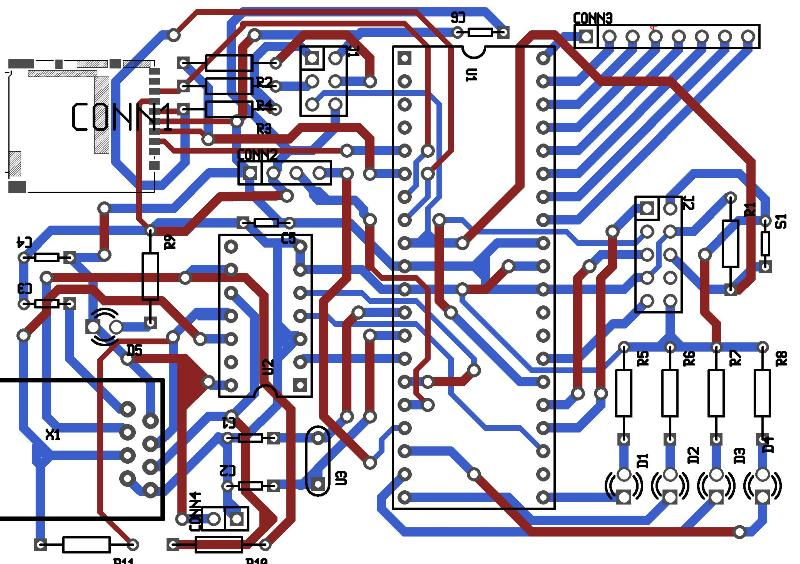
\includegraphics[width=1.0\textwidth, angle=90]{schematics/payload_644_layout.jpg}
\caption{Layout of our delivered PCB module. Dark Red: component layer. Light Blue: solder layer}
\end{figure}
